\subsubsection{\'Equilibrage automatique NUMA}

L'équilibrage automatique des pages mémoires ne donne pas de bonnes performances sur la factorisation (Fig.~\ref{fig:res_facto_frep}).
%
Cette méthode d'allocation est la moins efficace de toutes.
%
Avec un nombre suffisant d'itérations, l'allocation interleave donne les mêmes performances que l'allocation first touch.
%
L'utilisation de NATaS reste la solution qui donne les meilleurs performances.


%   (-_-)   %
\begin{figure}
  \centering
  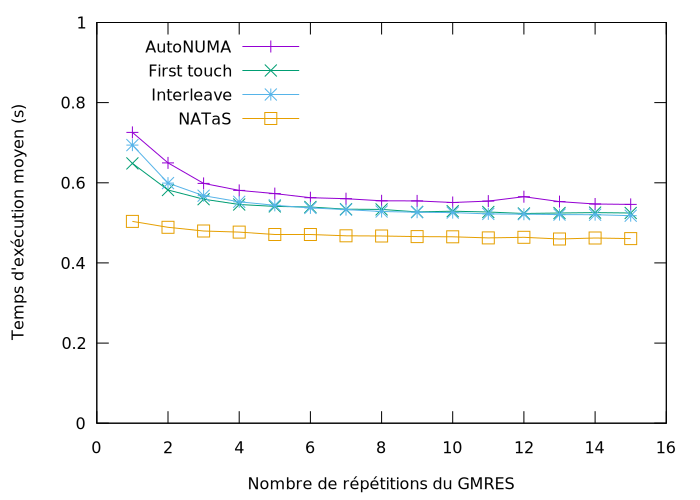
\includegraphics[width=0.7\textwidth]{res_facto_frep}
  \caption{Temps moyen d'une factorisation sur Linux 3.18 en mémoire partagée. Nous utilisons une matrice représentant un cube 100 avec 8 variables primaires.}
  \label{fig:res_facto_frep}
\end{figure}

Par contre, la résolution triangulaire se comporte comme le SpMV (Fig.~\ref{fig:res_trsv_frep}).
%
La politique d'allocation autoNUMA offre des performances intermédiaires aux politiques d'allocations first touch et interleave.
%
Encore une fois, l'utilisation de NATaS est la plus efficace.


%   (-_-)   %
\begin{figure}
  \centering
  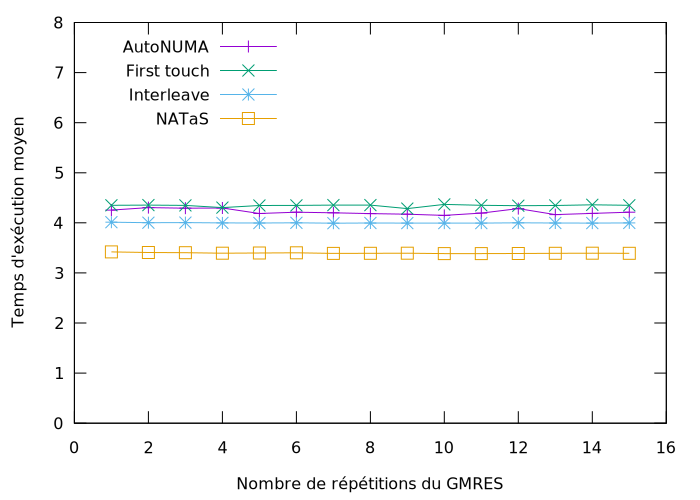
\includegraphics[width=0.7\textwidth]{res_trsv_frep}
  \caption{Temps moyen d'une résolution triangulaire sur Linux 3.18 en mémoire partagée. Nous utilisons une matrice représentant un cube 100 avec 8 variables primaires.}
  \label{fig:res_trsv_frep}
\end{figure}
